\mbox{$\displaystyle -\,$\,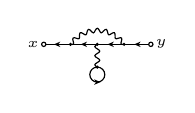
\begin{tikzpicture}[x=0.340cm, y=0.340cm, line width=0.420pt, baseline={([yshift=-0.6ex]0,0)}]
  \draw (-1.000,0.000) -- (-2.000,0.000);
  \fill (-1.619,0.000) -- (-1.381,-0.102) -- (-1.458,0.000) -- (-1.381,0.102) -- cycle;
  \draw (2.000,0.000) -- (1.000,0.000);
  \fill (1.381,0.000) -- (1.619,-0.102) -- (1.542,0.000) -- (1.619,0.102) -- cycle;
  \draw (0.000,0.000) -- (-1.000,0.000);
  \fill (-0.619,0.000) -- (-0.381,-0.102) -- (-0.458,0.000) -- (-0.381,0.102) -- cycle;
  \draw (1.000,0.000) -- (0.000,0.000);
  \fill (0.381,0.000) -- (0.619,-0.102) -- (0.542,0.000) -- (0.619,0.102) -- cycle;
  \draw plot[smooth, tension=0.7] coordinates {(0.000,-0.850) (-0.065,-0.808) (-0.092,-0.765) (-0.065,-0.722) (0.000,-0.680) (0.065,-0.638) (0.092,-0.595) (0.065,-0.552) (0.000,-0.510) (-0.065,-0.467) (-0.092,-0.425) (-0.065,-0.382) (0.000,-0.340) (0.065,-0.298) (0.092,-0.255) (0.065,-0.213) (0.000,-0.170) (-0.065,-0.127) (-0.092,-0.085) (-0.065,-0.042) (0.000,0.000)};
  \draw plot[smooth, tension=0.7] coordinates {(1.000,0.000) (0.931,-0.003) (0.890,0.012) (0.885,0.055) (0.902,0.122) (0.917,0.190) (0.904,0.236) (0.858,0.247) (0.790,0.230) (0.724,0.210) (0.680,0.214) (0.664,0.254) (0.665,0.323) (0.661,0.393) (0.638,0.434) (0.590,0.433) (0.529,0.400) (0.470,0.363) (0.427,0.356) (0.401,0.391) (0.384,0.458) (0.363,0.525) (0.330,0.559) (0.284,0.546) (0.233,0.498) (0.185,0.448) (0.145,0.429) (0.111,0.457) (0.078,0.518) (0.041,0.577) (0.000,0.601) (-0.041,0.577) (-0.078,0.518) (-0.111,0.457) (-0.145,0.429) (-0.185,0.448) (-0.233,0.498) (-0.284,0.546) (-0.330,0.559) (-0.363,0.525) (-0.384,0.458) (-0.401,0.391) (-0.427,0.356) (-0.470,0.363) (-0.529,0.400) (-0.590,0.433) (-0.638,0.434) (-0.661,0.393) (-0.665,0.323) (-0.664,0.254) (-0.680,0.214) (-0.724,0.210) (-0.790,0.230) (-0.858,0.247) (-0.904,0.236) (-0.917,0.190) (-0.902,0.122) (-0.885,0.055) (-0.890,0.012) (-0.931,-0.003) (-1.000,0.000)};
  \draw (0.000,-0.850) arc[start angle=90.000, end angle=450.000, radius=0.280];
  \fill (0.119,-1.410) -- (-0.119,-1.308) -- (-0.042,-1.410) -- (-0.119,-1.512) -- cycle;
  \fill (0.000,-0.850) circle (0.064);
  \fill (1.000,0.000) circle (0.064);
  \fill (-1.000,0.000) circle (0.064);
  \fill (0.000,0.000) circle (0.064);
  \draw[fill=white] (-2.000,0.000) circle (0.080);
  \draw[fill=white] (2.000,0.000) circle (0.080);
  \node[font=\tiny, inner sep=0pt, anchor=0] at (-2.170,0.000) {$x$};
  \node[font=\tiny, inner sep=0pt, anchor=180] at (2.170,0.000) {$y$};
\end{tikzpicture}}
\diagramgap
\mbox{$\displaystyle +\,$\,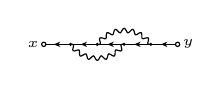
\begin{tikzpicture}[x=0.340cm, y=0.340cm, line width=0.420pt, baseline={([yshift=-0.6ex]0,0)}]
  \draw (-1.500,0.000) -- (-2.500,0.000);
  \fill (-2.119,0.000) -- (-1.881,-0.102) -- (-1.958,0.000) -- (-1.881,0.102) -- cycle;
  \draw (2.500,0.000) -- (1.500,0.000);
  \fill (1.881,0.000) -- (2.119,-0.102) -- (2.042,0.000) -- (2.119,0.102) -- cycle;
  \draw (-0.500,0.000) -- (-1.500,0.000);
  \fill (-1.119,0.000) -- (-0.881,-0.102) -- (-0.958,0.000) -- (-0.881,0.102) -- cycle;
  \draw (1.500,0.000) -- (0.500,0.000);
  \fill (0.881,0.000) -- (1.119,-0.102) -- (1.042,0.000) -- (1.119,0.102) -- cycle;
  \draw (0.500,0.000) -- (-0.500,0.000);
  \fill (-0.119,0.000) -- (0.119,-0.102) -- (0.042,0.000) -- (0.119,0.102) -- cycle;
  \draw plot[smooth, tension=0.7] coordinates {(1.500,0.000) (1.431,-0.003) (1.390,0.012) (1.385,0.055) (1.402,0.122) (1.417,0.190) (1.404,0.236) (1.358,0.247) (1.290,0.230) (1.224,0.210) (1.180,0.214) (1.164,0.254) (1.165,0.323) (1.161,0.393) (1.138,0.434) (1.090,0.433) (1.029,0.400) (0.970,0.363) (0.927,0.356) (0.901,0.391) (0.884,0.458) (0.863,0.525) (0.830,0.559) (0.784,0.546) (0.733,0.498) (0.685,0.448) (0.645,0.429) (0.611,0.457) (0.578,0.518) (0.541,0.577) (0.500,0.601) (0.459,0.577) (0.422,0.518) (0.389,0.457) (0.355,0.429) (0.315,0.448) (0.267,0.498) (0.216,0.546) (0.170,0.559) (0.137,0.525) (0.116,0.458) (0.099,0.391) (0.073,0.356) (0.030,0.363) (-0.029,0.400) (-0.090,0.433) (-0.138,0.434) (-0.161,0.393) (-0.165,0.323) (-0.164,0.254) (-0.180,0.214) (-0.224,0.210) (-0.290,0.230) (-0.358,0.247) (-0.404,0.236) (-0.417,0.190) (-0.402,0.122) (-0.385,0.055) (-0.390,0.012) (-0.431,-0.003) (-0.500,0.000)};
  \draw plot[smooth, tension=0.7] coordinates {(-1.500,0.000) (-1.431,0.003) (-1.390,-0.012) (-1.385,-0.055) (-1.402,-0.122) (-1.417,-0.190) (-1.404,-0.236) (-1.358,-0.247) (-1.290,-0.230) (-1.224,-0.210) (-1.180,-0.214) (-1.164,-0.254) (-1.165,-0.323) (-1.161,-0.393) (-1.138,-0.434) (-1.090,-0.433) (-1.029,-0.400) (-0.970,-0.363) (-0.927,-0.356) (-0.901,-0.391) (-0.884,-0.458) (-0.863,-0.525) (-0.830,-0.559) (-0.784,-0.546) (-0.733,-0.498) (-0.685,-0.448) (-0.645,-0.429) (-0.611,-0.457) (-0.578,-0.518) (-0.541,-0.577) (-0.500,-0.601) (-0.459,-0.577) (-0.422,-0.518) (-0.389,-0.457) (-0.355,-0.429) (-0.315,-0.448) (-0.267,-0.498) (-0.216,-0.546) (-0.170,-0.559) (-0.137,-0.525) (-0.116,-0.458) (-0.099,-0.391) (-0.073,-0.356) (-0.030,-0.363) (0.029,-0.400) (0.090,-0.433) (0.138,-0.434) (0.161,-0.393) (0.165,-0.323) (0.164,-0.254) (0.180,-0.214) (0.224,-0.210) (0.290,-0.230) (0.358,-0.247) (0.404,-0.236) (0.417,-0.190) (0.402,-0.122) (0.385,-0.055) (0.390,-0.012) (0.431,0.003) (0.500,0.000)};
  \fill (1.500,0.000) circle (0.064);
  \fill (-1.500,0.000) circle (0.064);
  \fill (0.500,0.000) circle (0.064);
  \fill (-0.500,0.000) circle (0.064);
  \draw[fill=white] (-2.500,0.000) circle (0.080);
  \draw[fill=white] (2.500,0.000) circle (0.080);
  \node[font=\tiny, inner sep=0pt, anchor=0] at (-2.670,0.000) {$x$};
  \node[font=\tiny, inner sep=0pt, anchor=180] at (2.670,0.000) {$y$};
\end{tikzpicture}}
\diagramgap
\mbox{$\displaystyle -\,$\,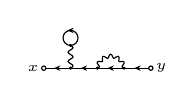
\begin{tikzpicture}[x=0.340cm, y=0.340cm, line width=0.420pt, baseline={([yshift=-0.6ex]0,0)}]
  \draw (-1.000,0.000) -- (-2.000,0.000);
  \fill (-1.619,0.000) -- (-1.381,-0.102) -- (-1.458,0.000) -- (-1.381,0.102) -- cycle;
  \draw (2.000,0.000) -- (1.000,0.000);
  \fill (1.381,0.000) -- (1.619,-0.102) -- (1.542,0.000) -- (1.619,0.102) -- cycle;
  \draw (0.000,0.000) -- (-1.000,0.000);
  \fill (-0.619,0.000) -- (-0.381,-0.102) -- (-0.458,0.000) -- (-0.381,0.102) -- cycle;
  \draw (1.000,0.000) -- (0.000,0.000);
  \fill (0.381,0.000) -- (0.619,-0.102) -- (0.542,0.000) -- (0.619,0.102) -- cycle;
  \draw plot[smooth, tension=0.7] coordinates {(1.000,0.000) (0.947,0.025) (0.921,0.050) (0.933,0.083) (0.968,0.130) (1.000,0.181) (1.001,0.224) (0.964,0.246) (0.904,0.247) (0.845,0.241) (0.811,0.249) (0.803,0.284) (0.811,0.342) (0.812,0.403) (0.791,0.440) (0.748,0.440) (0.696,0.410) (0.648,0.376) (0.614,0.365) (0.590,0.392) (0.567,0.446) (0.537,0.498) (0.500,0.520) (0.463,0.498) (0.433,0.446) (0.410,0.392) (0.386,0.365) (0.352,0.376) (0.304,0.410) (0.252,0.440) (0.209,0.440) (0.188,0.403) (0.189,0.342) (0.197,0.284) (0.189,0.249) (0.155,0.241) (0.096,0.247) (0.036,0.246) (-0.001,0.224) (0.000,0.181) (0.032,0.130) (0.067,0.083) (0.079,0.050) (0.053,0.025) (0.000,0.000)};
  \draw plot[smooth, tension=0.7] coordinates {(-1.000,0.850) (-0.935,0.808) (-0.908,0.765) (-0.935,0.722) (-1.000,0.680) (-1.065,0.638) (-1.092,0.595) (-1.065,0.552) (-1.000,0.510) (-0.935,0.467) (-0.908,0.425) (-0.935,0.382) (-1.000,0.340) (-1.065,0.298) (-1.092,0.255) (-1.065,0.213) (-1.000,0.170) (-0.935,0.127) (-0.908,0.085) (-0.935,0.042) (-1.000,0.000)};
  \draw (-1.000,0.850) arc[start angle=270.000, end angle=630.000, radius=0.280];
  \fill (-1.119,1.410) -- (-0.881,1.308) -- (-0.958,1.410) -- (-0.881,1.512) -- cycle;
  \fill (-1.000,0.850) circle (0.064);
  \fill (1.000,0.000) circle (0.064);
  \fill (-1.000,0.000) circle (0.064);
  \fill (0.000,0.000) circle (0.064);
  \draw[fill=white] (-2.000,0.000) circle (0.080);
  \draw[fill=white] (2.000,0.000) circle (0.080);
  \node[font=\tiny, inner sep=0pt, anchor=0] at (-2.170,0.000) {$x$};
  \node[font=\tiny, inner sep=0pt, anchor=180] at (2.170,0.000) {$y$};
\end{tikzpicture}}
\diagramgap
\mbox{$\displaystyle +\,$\,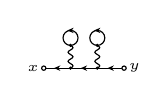
\begin{tikzpicture}[x=0.340cm, y=0.340cm, line width=0.420pt, baseline={([yshift=-0.6ex]0,0)}]
  \draw (-0.500,0.000) -- (-1.500,0.000);
  \fill (-1.119,0.000) -- (-0.881,-0.102) -- (-0.958,0.000) -- (-0.881,0.102) -- cycle;
  \draw (1.500,0.000) -- (0.500,0.000);
  \fill (0.881,0.000) -- (1.119,-0.102) -- (1.042,0.000) -- (1.119,0.102) -- cycle;
  \draw (0.500,0.000) -- (-0.500,0.000);
  \fill (-0.119,0.000) -- (0.119,-0.102) -- (0.042,0.000) -- (0.119,0.102) -- cycle;
  \draw plot[smooth, tension=0.7] coordinates {(0.500,0.850) (0.565,0.808) (0.592,0.765) (0.565,0.722) (0.500,0.680) (0.435,0.638) (0.408,0.595) (0.435,0.552) (0.500,0.510) (0.565,0.467) (0.592,0.425) (0.565,0.382) (0.500,0.340) (0.435,0.298) (0.408,0.255) (0.435,0.213) (0.500,0.170) (0.565,0.127) (0.592,0.085) (0.565,0.042) (0.500,0.000)};
  \draw plot[smooth, tension=0.7] coordinates {(-0.500,0.850) (-0.435,0.808) (-0.408,0.765) (-0.435,0.722) (-0.500,0.680) (-0.565,0.638) (-0.592,0.595) (-0.565,0.552) (-0.500,0.510) (-0.435,0.467) (-0.408,0.425) (-0.435,0.382) (-0.500,0.340) (-0.565,0.298) (-0.592,0.255) (-0.565,0.213) (-0.500,0.170) (-0.435,0.127) (-0.408,0.085) (-0.435,0.042) (-0.500,0.000)};
  \draw (0.500,0.850) arc[start angle=270.000, end angle=630.000, radius=0.280];
  \fill (0.381,1.410) -- (0.619,1.308) -- (0.542,1.410) -- (0.619,1.512) -- cycle;
  \draw (-0.500,0.850) arc[start angle=270.000, end angle=630.000, radius=0.280];
  \fill (-0.619,1.410) -- (-0.381,1.308) -- (-0.458,1.410) -- (-0.381,1.512) -- cycle;
  \fill (0.500,0.850) circle (0.064);
  \fill (-0.500,0.850) circle (0.064);
  \fill (0.500,0.000) circle (0.064);
  \fill (-0.500,0.000) circle (0.064);
  \draw[fill=white] (-1.500,0.000) circle (0.080);
  \draw[fill=white] (1.500,0.000) circle (0.080);
  \node[font=\tiny, inner sep=0pt, anchor=0] at (-1.670,0.000) {$x$};
  \node[font=\tiny, inner sep=0pt, anchor=180] at (1.670,0.000) {$y$};
\end{tikzpicture}}
\diagramgap
\mbox{$\displaystyle +\,$\,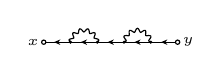
\begin{tikzpicture}[x=0.340cm, y=0.340cm, line width=0.420pt, baseline={([yshift=-0.6ex]0,0)}]
  \draw (-1.500,0.000) -- (-2.500,0.000);
  \fill (-2.119,0.000) -- (-1.881,-0.102) -- (-1.958,0.000) -- (-1.881,0.102) -- cycle;
  \draw (2.500,0.000) -- (1.500,0.000);
  \fill (1.881,0.000) -- (2.119,-0.102) -- (2.042,0.000) -- (2.119,0.102) -- cycle;
  \draw (-0.500,0.000) -- (-1.500,0.000);
  \fill (-1.119,0.000) -- (-0.881,-0.102) -- (-0.958,0.000) -- (-0.881,0.102) -- cycle;
  \draw plot[smooth, tension=0.7] coordinates {(-1.500,0.000) (-1.544,0.042) (-1.556,0.082) (-1.527,0.113) (-1.468,0.130) (-1.411,0.140) (-1.379,0.157) (-1.381,0.193) (-1.404,0.247) (-1.421,0.305) (-1.410,0.346) (-1.369,0.358) (-1.311,0.342) (-1.256,0.322) (-1.220,0.320) (-1.204,0.352) (-1.196,0.410) (-1.181,0.469) (-1.151,0.499) (-1.110,0.488) (-1.067,0.446) (-1.030,0.400) (-1.000,0.380) (-0.970,0.400) (-0.933,0.446) (-0.890,0.488) (-0.849,0.499) (-0.819,0.469) (-0.804,0.410) (-0.796,0.352) (-0.780,0.320) (-0.744,0.322) (-0.689,0.342) (-0.631,0.358) (-0.590,0.346) (-0.579,0.305) (-0.596,0.247) (-0.619,0.193) (-0.621,0.157) (-0.589,0.140) (-0.532,0.130) (-0.473,0.113) (-0.444,0.082) (-0.456,0.042) (-0.500,0.000)};
  \draw (1.500,0.000) -- (0.500,0.000);
  \fill (0.881,0.000) -- (1.119,-0.102) -- (1.042,0.000) -- (1.119,0.102) -- cycle;
  \draw plot[smooth, tension=0.7] coordinates {(1.500,0.000) (1.447,0.025) (1.421,0.050) (1.433,0.083) (1.468,0.130) (1.500,0.181) (1.501,0.224) (1.464,0.246) (1.404,0.247) (1.345,0.241) (1.311,0.249) (1.303,0.284) (1.311,0.342) (1.312,0.403) (1.291,0.440) (1.248,0.440) (1.196,0.410) (1.148,0.376) (1.114,0.365) (1.090,0.392) (1.067,0.446) (1.037,0.498) (1.000,0.520) (0.963,0.498) (0.933,0.446) (0.910,0.392) (0.886,0.365) (0.852,0.376) (0.804,0.410) (0.752,0.440) (0.709,0.440) (0.688,0.403) (0.689,0.342) (0.697,0.284) (0.689,0.249) (0.655,0.241) (0.596,0.247) (0.536,0.246) (0.499,0.224) (0.500,0.181) (0.532,0.130) (0.567,0.083) (0.579,0.050) (0.553,0.025) (0.500,0.000)};
  \draw (0.500,0.000) -- (-0.500,0.000);
  \fill (-0.119,0.000) -- (0.119,-0.102) -- (0.042,0.000) -- (0.119,0.102) -- cycle;
  \fill (1.500,0.000) circle (0.064);
  \fill (-1.500,0.000) circle (0.064);
  \fill (0.500,0.000) circle (0.064);
  \fill (-0.500,0.000) circle (0.064);
  \draw[fill=white] (-2.500,0.000) circle (0.080);
  \draw[fill=white] (2.500,0.000) circle (0.080);
  \node[font=\tiny, inner sep=0pt, anchor=0] at (-2.670,0.000) {$x$};
  \node[font=\tiny, inner sep=0pt, anchor=180] at (2.670,0.000) {$y$};
\end{tikzpicture}}
\diagramgap
\mbox{$\displaystyle +\,$\,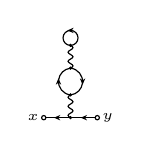
\begin{tikzpicture}[x=0.340cm, y=0.340cm, line width=0.420pt, baseline={([yshift=-0.6ex]0,0)}]
  \draw (0.000,0.000) -- (-1.000,0.000);
  \fill (-0.619,0.000) -- (-0.381,-0.102) -- (-0.458,0.000) -- (-0.381,0.102) -- cycle;
  \draw (1.000,0.000) -- (0.000,0.000);
  \fill (0.381,0.000) -- (0.619,-0.102) -- (0.542,0.000) -- (0.619,0.102) -- cycle;
  \draw (0.000,0.850) arc[start angle=263.974, end angle=96.026, radius=0.503];
  \fill (-0.450,1.469) -- (-0.552,1.231) -- (-0.450,1.308) -- (-0.348,1.231) -- cycle;
  \draw (0.000,1.850) arc[start angle=83.974, end angle=-83.974, radius=0.503];
  \fill (0.450,1.231) -- (0.552,1.469) -- (0.450,1.392) -- (0.348,1.469) -- cycle;
  \draw plot[smooth, tension=0.7] coordinates {(0.000,2.700) (0.065,2.658) (0.092,2.615) (0.065,2.573) (0.000,2.530) (-0.065,2.488) (-0.092,2.445) (-0.065,2.403) (0.000,2.360) (0.065,2.318) (0.092,2.275) (0.065,2.232) (0.000,2.190) (-0.065,2.148) (-0.092,2.105) (-0.065,2.062) (0.000,2.020) (0.065,1.978) (0.092,1.935) (0.065,1.892) (0.000,1.850)};
  \draw plot[smooth, tension=0.7] coordinates {(0.000,0.000) (-0.065,0.042) (-0.092,0.085) (-0.065,0.128) (0.000,0.170) (0.065,0.212) (0.092,0.255) (0.065,0.298) (0.000,0.340) (-0.065,0.382) (-0.092,0.425) (-0.065,0.468) (0.000,0.510) (0.065,0.552) (0.092,0.595) (0.065,0.638) (0.000,0.680) (-0.065,0.722) (-0.092,0.765) (-0.065,0.808) (0.000,0.850)};
  \draw (0.000,2.700) arc[start angle=270.000, end angle=630.000, radius=0.280];
  \fill (-0.119,3.260) -- (0.119,3.158) -- (0.042,3.260) -- (0.119,3.362) -- cycle;
  \fill (0.000,2.700) circle (0.064);
  \fill (0.000,0.000) circle (0.064);
  \fill (0.000,1.850) circle (0.064);
  \fill (0.000,0.850) circle (0.064);
  \draw[fill=white] (-1.000,0.000) circle (0.080);
  \draw[fill=white] (1.000,0.000) circle (0.080);
  \node[font=\tiny, inner sep=0pt, anchor=0] at (-1.170,0.000) {$x$};
  \node[font=\tiny, inner sep=0pt, anchor=180] at (1.170,0.000) {$y$};
\end{tikzpicture}}
\diagramgap
\mbox{$\displaystyle -\,$\,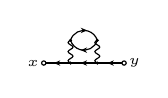
\begin{tikzpicture}[x=0.340cm, y=0.340cm, line width=0.420pt, baseline={([yshift=-0.6ex]0,0)}]
  \draw (-0.500,0.000) -- (-1.500,0.000);
  \fill (-1.119,0.000) -- (-0.881,-0.102) -- (-0.958,0.000) -- (-0.881,0.102) -- cycle;
  \draw (1.500,0.000) -- (0.500,0.000);
  \fill (0.881,0.000) -- (1.119,-0.102) -- (1.042,0.000) -- (1.119,0.102) -- cycle;
  \draw (0.500,0.000) -- (-0.500,0.000);
  \fill (-0.119,0.000) -- (0.119,-0.102) -- (0.042,0.000) -- (0.119,0.102) -- cycle;
  \draw (-0.500,0.850) arc[start angle=162.811, end angle=17.189, radius=0.523];
  \fill (0.119,1.219) -- (-0.119,1.321) -- (-0.042,1.219) -- (-0.119,1.117) -- cycle;
  \draw (0.500,0.850) arc[start angle=342.811, end angle=197.189, radius=0.523];
  \fill (-0.119,0.481) -- (0.119,0.379) -- (0.042,0.481) -- (0.119,0.583) -- cycle;
  \draw plot[smooth, tension=0.7] coordinates {(0.500,0.000) (0.435,0.042) (0.408,0.085) (0.435,0.128) (0.500,0.170) (0.565,0.212) (0.592,0.255) (0.565,0.298) (0.500,0.340) (0.435,0.382) (0.408,0.425) (0.435,0.468) (0.500,0.510) (0.565,0.552) (0.592,0.595) (0.565,0.638) (0.500,0.680) (0.435,0.722) (0.408,0.765) (0.435,0.808) (0.500,0.850)};
  \draw plot[smooth, tension=0.7] coordinates {(-0.500,0.000) (-0.565,0.042) (-0.592,0.085) (-0.565,0.128) (-0.500,0.170) (-0.435,0.212) (-0.408,0.255) (-0.435,0.298) (-0.500,0.340) (-0.565,0.382) (-0.592,0.425) (-0.565,0.468) (-0.500,0.510) (-0.435,0.552) (-0.408,0.595) (-0.435,0.638) (-0.500,0.680) (-0.565,0.722) (-0.592,0.765) (-0.565,0.808) (-0.500,0.850)};
  \fill (0.500,0.000) circle (0.064);
  \fill (-0.500,0.000) circle (0.064);
  \fill (0.500,0.850) circle (0.064);
  \fill (-0.500,0.850) circle (0.064);
  \draw[fill=white] (-1.500,0.000) circle (0.080);
  \draw[fill=white] (1.500,0.000) circle (0.080);
  \node[font=\tiny, inner sep=0pt, anchor=0] at (-1.670,0.000) {$x$};
  \node[font=\tiny, inner sep=0pt, anchor=180] at (1.670,0.000) {$y$};
\end{tikzpicture}}
\diagramgap
\mbox{$\displaystyle -\,$\,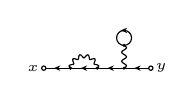
\begin{tikzpicture}[x=0.340cm, y=0.340cm, line width=0.420pt, baseline={([yshift=-0.6ex]0,0)}]
  \draw (-1.000,0.000) -- (-2.000,0.000);
  \fill (-1.619,0.000) -- (-1.381,-0.102) -- (-1.458,0.000) -- (-1.381,0.102) -- cycle;
  \draw (2.000,0.000) -- (1.000,0.000);
  \fill (1.381,0.000) -- (1.619,-0.102) -- (1.542,0.000) -- (1.619,0.102) -- cycle;
  \draw (0.000,0.000) -- (-1.000,0.000);
  \fill (-0.619,0.000) -- (-0.381,-0.102) -- (-0.458,0.000) -- (-0.381,0.102) -- cycle;
  \draw plot[smooth, tension=0.7] coordinates {(-1.000,0.000) (-1.044,0.042) (-1.056,0.082) (-1.027,0.113) (-0.968,0.130) (-0.911,0.140) (-0.879,0.157) (-0.881,0.193) (-0.904,0.247) (-0.921,0.305) (-0.910,0.346) (-0.869,0.358) (-0.811,0.342) (-0.756,0.322) (-0.720,0.320) (-0.704,0.352) (-0.696,0.410) (-0.681,0.469) (-0.651,0.499) (-0.610,0.488) (-0.567,0.446) (-0.530,0.400) (-0.500,0.380) (-0.470,0.400) (-0.433,0.446) (-0.390,0.488) (-0.349,0.499) (-0.319,0.469) (-0.304,0.410) (-0.296,0.352) (-0.280,0.320) (-0.244,0.322) (-0.189,0.342) (-0.131,0.358) (-0.090,0.346) (-0.079,0.305) (-0.096,0.247) (-0.119,0.193) (-0.121,0.157) (-0.089,0.140) (-0.032,0.130) (0.027,0.113) (0.056,0.082) (0.044,0.042) (0.000,0.000)};
  \draw (1.000,0.000) -- (0.000,0.000);
  \fill (0.381,0.000) -- (0.619,-0.102) -- (0.542,0.000) -- (0.619,0.102) -- cycle;
  \draw plot[smooth, tension=0.7] coordinates {(1.000,0.850) (1.065,0.808) (1.092,0.765) (1.065,0.722) (1.000,0.680) (0.935,0.638) (0.908,0.595) (0.935,0.552) (1.000,0.510) (1.065,0.467) (1.092,0.425) (1.065,0.382) (1.000,0.340) (0.935,0.298) (0.908,0.255) (0.935,0.213) (1.000,0.170) (1.065,0.127) (1.092,0.085) (1.065,0.042) (1.000,0.000)};
  \draw (1.000,0.850) arc[start angle=270.000, end angle=630.000, radius=0.280];
  \fill (0.881,1.410) -- (1.119,1.308) -- (1.042,1.410) -- (1.119,1.512) -- cycle;
  \fill (1.000,0.850) circle (0.064);
  \fill (1.000,0.000) circle (0.064);
  \fill (-1.000,0.000) circle (0.064);
  \fill (0.000,0.000) circle (0.064);
  \draw[fill=white] (-2.000,0.000) circle (0.080);
  \draw[fill=white] (2.000,0.000) circle (0.080);
  \node[font=\tiny, inner sep=0pt, anchor=0] at (-2.170,0.000) {$x$};
  \node[font=\tiny, inner sep=0pt, anchor=180] at (2.170,0.000) {$y$};
\end{tikzpicture}}
\diagramgap
\mbox{$\displaystyle +\,$\,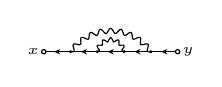
\begin{tikzpicture}[x=0.340cm, y=0.340cm, line width=0.420pt, baseline={([yshift=-0.6ex]0,0)}]
  \draw (-1.500,0.000) -- (-2.500,0.000);
  \fill (-2.119,0.000) -- (-1.881,-0.102) -- (-1.958,0.000) -- (-1.881,0.102) -- cycle;
  \draw (2.500,0.000) -- (1.500,0.000);
  \fill (1.881,0.000) -- (2.119,-0.102) -- (2.042,0.000) -- (2.119,0.102) -- cycle;
  \draw (-0.500,0.000) -- (-1.500,0.000);
  \fill (-1.119,0.000) -- (-0.881,-0.102) -- (-0.958,0.000) -- (-0.881,0.102) -- cycle;
  \draw (1.500,0.000) -- (0.500,0.000);
  \fill (0.881,0.000) -- (1.119,-0.102) -- (1.042,0.000) -- (1.119,0.102) -- cycle;
  \draw (0.500,0.000) -- (-0.500,0.000);
  \fill (-0.119,0.000) -- (0.119,-0.102) -- (0.042,0.000) -- (0.119,0.102) -- cycle;
  \draw plot[smooth, tension=0.7] coordinates {(0.500,0.000) (0.447,0.025) (0.421,0.050) (0.433,0.083) (0.468,0.130) (0.500,0.181) (0.501,0.224) (0.464,0.246) (0.404,0.247) (0.345,0.241) (0.311,0.249) (0.303,0.284) (0.311,0.342) (0.312,0.403) (0.291,0.440) (0.248,0.440) (0.196,0.410) (0.148,0.376) (0.114,0.365) (0.090,0.392) (0.067,0.446) (0.037,0.498) (0.000,0.520) (-0.037,0.498) (-0.067,0.446) (-0.090,0.392) (-0.114,0.365) (-0.148,0.376) (-0.196,0.410) (-0.248,0.440) (-0.291,0.440) (-0.312,0.403) (-0.311,0.342) (-0.303,0.284) (-0.311,0.249) (-0.345,0.241) (-0.404,0.247) (-0.464,0.246) (-0.501,0.224) (-0.500,0.181) (-0.468,0.130) (-0.433,0.083) (-0.421,0.050) (-0.447,0.025) (-0.500,0.000)};
  \draw plot[smooth, tension=0.7] coordinates {(1.500,0.000) (1.418,-0.003) (1.369,0.015) (1.364,0.067) (1.386,0.146) (1.406,0.226) (1.394,0.281) (1.340,0.295) (1.259,0.279) (1.179,0.260) (1.127,0.268) (1.111,0.318) (1.118,0.399) (1.121,0.482) (1.098,0.533) (1.042,0.537) (0.966,0.505) (0.892,0.470) (0.840,0.467) (0.814,0.513) (0.804,0.594) (0.791,0.676) (0.758,0.721) (0.702,0.713) (0.634,0.667) (0.569,0.618) (0.518,0.605) (0.484,0.644) (0.458,0.722) (0.428,0.799) (0.387,0.837) (0.334,0.818) (0.276,0.759) (0.222,0.698) (0.175,0.675) (0.133,0.707) (0.092,0.778) (0.048,0.847) (0.000,0.876) (-0.048,0.847) (-0.092,0.778) (-0.133,0.707) (-0.175,0.675) (-0.222,0.698) (-0.276,0.759) (-0.334,0.818) (-0.387,0.837) (-0.428,0.799) (-0.458,0.722) (-0.484,0.644) (-0.518,0.605) (-0.569,0.618) (-0.634,0.667) (-0.702,0.713) (-0.758,0.721) (-0.791,0.676) (-0.804,0.594) (-0.814,0.513) (-0.840,0.467) (-0.892,0.470) (-0.966,0.505) (-1.042,0.537) (-1.098,0.533) (-1.121,0.482) (-1.118,0.399) (-1.111,0.318) (-1.127,0.268) (-1.179,0.260) (-1.259,0.279) (-1.340,0.295) (-1.394,0.281) (-1.406,0.226) (-1.386,0.146) (-1.364,0.067) (-1.369,0.015) (-1.418,-0.003) (-1.500,0.000)};
  \fill (1.500,0.000) circle (0.064);
  \fill (-1.500,0.000) circle (0.064);
  \fill (0.500,0.000) circle (0.064);
  \fill (-0.500,0.000) circle (0.064);
  \draw[fill=white] (-2.500,0.000) circle (0.080);
  \draw[fill=white] (2.500,0.000) circle (0.080);
  \node[font=\tiny, inner sep=0pt, anchor=0] at (-2.670,0.000) {$x$};
  \node[font=\tiny, inner sep=0pt, anchor=180] at (2.670,0.000) {$y$};
\end{tikzpicture}}
\diagramgap
\mbox{$\displaystyle -\,$\,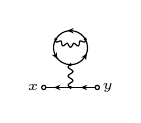
\begin{tikzpicture}[x=0.340cm, y=0.340cm, line width=0.420pt, baseline={([yshift=-0.6ex]0,0)}]
  \draw (0.000,0.000) -- (-1.000,0.000);
  \fill (-0.619,0.000) -- (-0.381,-0.102) -- (-0.458,0.000) -- (-0.381,0.102) -- cycle;
  \draw (1.000,0.000) -- (0.000,0.000);
  \fill (0.381,0.000) -- (0.619,-0.102) -- (0.542,0.000) -- (0.619,0.102) -- cycle;
  \draw (-0.550,1.803) arc[start angle=150.000, end angle=270.000, radius=0.635];
  \fill (-0.490,1.064) -- (-0.521,1.322) -- (-0.571,1.204) -- (-0.698,1.220) -- cycle;
  \draw (0.000,0.850) arc[start angle=270.000, end angle=390.000, radius=0.635];
  \fill (0.610,1.271) -- (0.402,1.115) -- (0.529,1.131) -- (0.579,1.013) -- cycle;
  \draw (0.550,1.803) arc[start angle=30.000, end angle=150.000, radius=0.635];
  \fill (-0.119,2.120) -- (0.119,2.018) -- (0.042,2.120) -- (0.119,2.222) -- cycle;
  \draw plot[smooth, tension=0.7] coordinates {(0.550,1.803) (0.560,1.742) (0.547,1.702) (0.505,1.695) (0.447,1.714) (0.391,1.737) (0.354,1.738) (0.337,1.704) (0.330,1.645) (0.318,1.585) (0.292,1.552) (0.250,1.559) (0.202,1.597) (0.158,1.638) (0.123,1.652) (0.095,1.627) (0.068,1.573) (0.036,1.521) (0.000,1.499) (-0.036,1.521) (-0.068,1.573) (-0.095,1.627) (-0.123,1.652) (-0.158,1.638) (-0.202,1.597) (-0.250,1.559) (-0.292,1.552) (-0.318,1.585) (-0.330,1.645) (-0.337,1.704) (-0.354,1.738) (-0.391,1.737) (-0.447,1.714) (-0.505,1.695) (-0.547,1.702) (-0.560,1.742) (-0.550,1.803)};
  \draw plot[smooth, tension=0.7] coordinates {(0.000,0.000) (-0.065,0.043) (-0.092,0.085) (-0.065,0.128) (0.000,0.170) (0.065,0.213) (0.092,0.255) (0.065,0.298) (0.000,0.340) (-0.065,0.383) (-0.092,0.425) (-0.065,0.468) (0.000,0.510) (0.065,0.553) (0.092,0.595) (0.065,0.638) (0.000,0.680) (-0.065,0.723) (-0.092,0.765) (-0.065,0.808) (0.000,0.850)};
  \fill (0.000,0.000) circle (0.064);
  \fill (0.000,0.850) circle (0.064);
  \fill (0.550,1.803) circle (0.064);
  \fill (-0.550,1.803) circle (0.064);
  \draw[fill=white] (-1.000,0.000) circle (0.080);
  \draw[fill=white] (1.000,0.000) circle (0.080);
  \node[font=\tiny, inner sep=0pt, anchor=0] at (-1.170,0.000) {$x$};
  \node[font=\tiny, inner sep=0pt, anchor=180] at (1.170,0.000) {$y$};
\end{tikzpicture}}
